% vim: textwidth=80
\documentclass[notitlepage]{article}

% packages
\usepackage[pdftex]{graphicx}
\usepackage{listings}
\usepackage{float}
\usepackage{titling}
\usepackage{subfigure}
\usepackage{url}
\usepackage{hyperref}

\graphicspath{{./figures/}}

% set the code to wrap and have box
\lstset{
    frame=single,
    breaklines=true
}

% move the title up
\setlength{\droptitle}{-10em}

\begin{document}

% title
\title{Senior Thesis Research Report}
\author{Raj Ramamurthy\\
  \texttt{rmmrthy2 @ illinois.edu}}
\maketitle


\section{Introduction}
This report summarizes my work with the DEPEND research group as part of CS499
(senior thesis) from January 2015 through December 2015.

The paper is structured as follows. A brief discussion of performance counters
work is provided in Section II. An overview of the userspace data is presented
in Section III. In Section IV, the development of the kernel module and
interaction with KVM is explained. Section V contains an overview of the data
collection and architecture. Section VI analyzes the data that was collected,
with areas for future work presented in Section VII. Finally, the conclusions
from this work are available in Section VIII.

\subsection{Timeline}
This project took place over two semesters. In the first semester, the initial
plan for the work was developed and several core components were engineered.
This includes the user space counter collection tool and the kernel space tool.

The second semester of this work was mostly focused around understanding whether
performance counters can be a useful invariant on thier own, or whetherother
components would need to be used in order to detect execution irregularities.
This involved collecting data, creating tools to analyze it, and graphing the
data to understand its usefulness.

\subsection{Background}
This thesis was grown out of previous semsters I had spent working with the
DEPEND research group. Specifically, in this work,  I sought to answer the
following question:
\textit{by constructing fingerprints
    from execution signatures (using performance counters) of a hypervisor
    (e.g., qemu-kvm) at different points in time, is it possible to detect
    compromised hypervisor execution by comparing them to known good ones?} This
    is a form of \textit{dynamic analysis} because the detection is done at
    runtime and not at compile time (static analysis).

\subsection{Hardware Performance Counters}
Hardware performance counters (herein referred to as HPCs) allow for the
collection of various low-level information about a processor's current state.
The counters can provide valuable performance insights. Unfortunately, the first
machine I attempted to use did not support HPCs, and it is not enabled by
default on most machines.  However, after switching to another machine, I was
able to enable the counters and begin collecting data.

The counters available vary from machine to machine. The important counters are
total retired instructions, conditional branch instructions, branch
instructions, store instructions, and load instructions.  The counters were
collected with PAPI, which is described in the next section.

\subsection{Motivation}
To understand the motivation behind this project, it is important to have a good
high-level understanding of the virtualized system topology. A visual overview
of the topology is shown in Figure~\ref{fig:vmtop}.

\begin{figure}[htp]
    \centering
    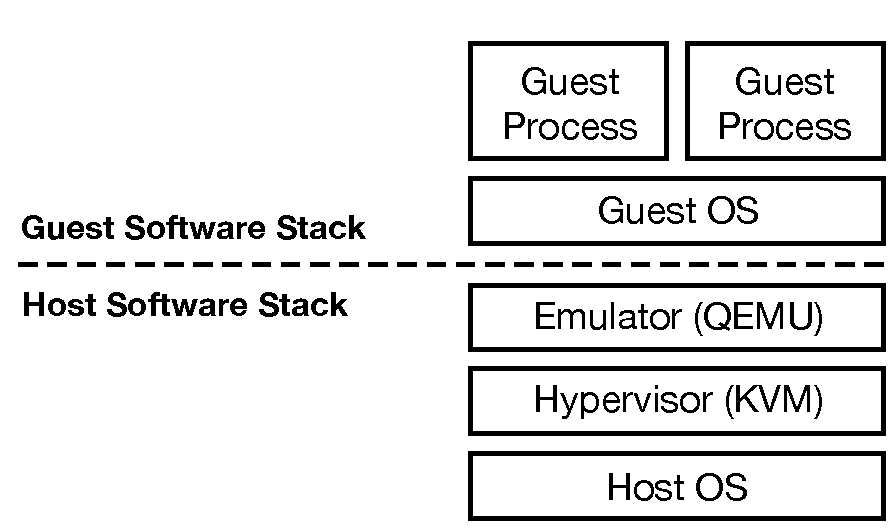
\includegraphics[width=3.5in]{container_diagram.pdf}
    \caption{Virtual machine topology. Areas of focus include QEMU and KVM.}
    \label{fig:vmtop}
\end{figure}

A search of the National Vulnerability Database shows that there are many
reported vulnerabilities in QEMU. These range in severity, but can be as grave
as allowing for arbitrary code execution by the virtual machine
guest.\footnote{\url{http://web.nvd.nist.gov/view/vuln/search-results?query=QEMU&search_type=all&cves=on}}
While there are research papers already published on dynamic analysis using
hardware performance counters, these have not been applied towards
virtualization\cite{numchecker}\cite{feasibility}\cite{pc}.

The principal motivation for this work was to understand if we could feasibly
develop a method of detecting a compromised hypervisor. Hypervisor security is
very important, and because the hypervisor functions as the backbone of a
virtualized system, its integrity is paramount for the virtual machine's
security.


\section{Related Work}
There are a number of existing works which cover HPCs for security. These center
around several concerns:
\begin{itemize}
    \item Overhead in using HPCs
    \item Accuracy and nondeterminism of the counters
    \item Accuracy of detection methods using counters
    \item Feasability of HPCs as a dynamic analysis invariant
\end{itemize}

\subsection{Using Counters for Dynamic Analysis}
The paper ``Are Hardware Performance Counters a Cost Effective Way for Integrity
Checking of Programs?'' attempts to understand performance counter usage for
integrity checking from a cost perspective, and concludes that HPCs are
efficient for detecting program modification\cite{arehardware}. The
NumChecker\cite{numchecker} paper presents a framework through which to detect
kernel rootkits. It uses HPCs to verify system call execution.

\subsection{Overhead}
As the name implies, hardware performance counters were initially designed to
aid in performance instrumentation of low-level software. Using HPCs is
attractive because they are built into the processor, meaning that they add a
negligible amount of hardware overhead to program execution. However, storing
this information and analyzing it dynamically can introduce overhead. The
NumChecker\cite{numchecker} paper reveals that the amount of overhead varies
significantly with the frequency of collection,  presumably due to I/O; for a
sampling rate of 5 seconds, the overhead introduced by NumChecker was
2.8\%\cite{numchecker}. Another work shows that the overhead incurred in that
situation was less than 10\%\cite{arehardware}.

\subsection{Counter Accuracy and Nondeterminism}
Using HPCs as an invariant has proved a controversial topic, as they appear to
be nondeterministic. This is because there are many events happening on the
processor, which cause small fluctuations in the counter values.

However, some metrics are more consistent than others. From \cite{arehardware}:
``The shortlisted events include the total number of instructions retired, the
number of branch instructions retired, cache stores (they are better measures
than loads because loads can be speculative), completed I/O operations, and
number of floating point operations.''\cite{arehardware}

There are many sources of nondeterminism, and it appears to vary from chip to
chip. The paper ``Non-determinism and overcount on modern hardware performance
counter implementations'' explores these sources and attempts to make sense of
which counters are best. It comes to the conclusion that total instructions
retired is one of the most consistent counters\cite{overcount}.

\subsection{Detection Accuracy from Using HPCs}
HPCs only provide the data. From this data, is important to conduct proper
statistical analysis to achieve meaningful results. Specifically, in integrity
checking, the most important metric is a low false positive rate.

The HPC data is best interpreted as a matrix of feature vectors.  From this, a
number of very interesting analytical techniques arise, including (but not
limited to): linear regression, support vector machines, random forests, nearest
neighbors, and clustering. Principally, nearest neighbors is the most popular of
these choices, but each approach has different advantages\cite{forsyth}. It is
also possible to build simple classification simply by looking within a
threshold of all known values\cite{numchecker}. In one paper, artificial neural
networks were used\cite{feasibility}.




\section{QEMU}
QEMU is a machine emulator which allows for the emulation of a platform so that
a full operating system/hypervisor may run on top of it. QEMU provides emulation
of both entire machines and external I/O devices (e.g., hard-drives, network
devices, and keyboards). However, when the host and guest operating system are
the same architecture\footnote{An \texttt{x86} machine may also be virtualized
on an \texttt{x86\_64} architecture}, native virtualization can be accomplished
by using KVM, a Linux kernel feature which allows for hardware-assisted
virtualization. KVM leverages processor support for virtualization to expose an
API for running guest virtual machines. In this configuration, QEMU only
emulates I/O devices.  Because both pieces of software play crucial roles in
running the guest virtual machine, execution frequently traps from one to
another. This is explained in Figure~\ref{fig:qemutrap}.

\begin{figure}
    \centering    
    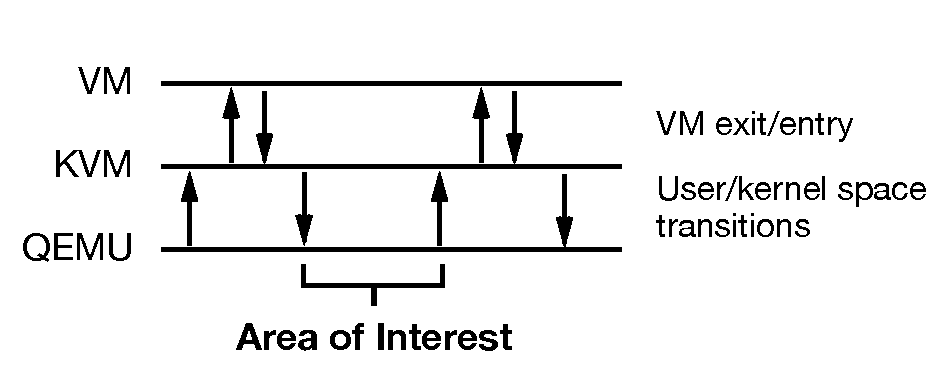
\includegraphics[width=4in]{qemu_trap.pdf}
    \caption{Diagram of the various transfers of control between QEMU, KVM, and
        the host virtual machine. When KVM returns to QEMU, it provides an exit
        reason which can be used by QEMU to take appropriate action. However,
        KVM may transfer control to the virtual machine (and back) before
        returning to QEMU. The arrows represent transfer of control. The
        duration for which HPCs were recorded is also displayed. The area of
        interest highlighted was chosen because it focuses solely on QEMU while
        allowing for collection of the exit reason from KVM.}
\label{fig:qemutrap}
\end{figure}

\subsection{Modifications}
In order to collect HPC data from QEMU, some modifications were required. QEMU
does not have a plugin architecture, so a custom build of QEMU was created for
instrumentation purposes.

The modifications were fairly simple: using the PAPI performance counter
library, I was able to output HPC measurements across a known path of execution.
Furthermore, with the KVM hypercall extension, I was able to make markings in
the data collection from within the guest VM. With this toolset, it became
trivial to mark the beginning and ending of a program in the guest VM and
observe the QEMU data for this period.


\section{KVM and \texttt{kprof}}
The KVM kernel module was modified for use in this project. This section aims to
explain the changes that were made and elaborate on the design of the additional
data collection module that was developed.\footnote{A full list of modifications
to the module is available in the README of the project.}

\subsection{KVM Exits}
When execution is transferred to the KVM context, the hypervisor will return
what is known as an \textit{exit reason} when execution transfers back. The exit
reason is related to the hardware VM exit provided by VT-x. There is
a long list of exit reasons spanning many different explanations for what
occurred while KVM had control of execution. \footnote{A full list of the exit
    reasons for KVM is available at
\url{http://lxr.free-electrons.com/source/arch/x86/include/uapi/asm/vmx.h\#L30}}

\subsection{The \texttt{kprof} Module}
In order to be able to collect the data from user space, I developed a device
driver. This allows the usage of the \texttt{ioctl} function from the user space
program (useragent) and for data to be transferred out of the kernel.

In the device driver, called \texttt{kprof}, a set of internal buffers in
constructed so that the data may be continuously populated in memory and then
flushed to disk at an interval (this is the same technique used in the hprobe
kernel module).  This helps keep the performance impact of this double buffer
solution manageable in addition to providing a lock-free mechanism for reading
the data from multiple code paths.

The current module exposes two simple symbols:
\begin{enumerate}
    \item{\texttt{start\_record()}, which starts the recording of events.}
    \item{\texttt{stop\_record(exit\_reason)}, which stops the recoding, records
        the difference since the last call to \texttt{start\_record}, and
    records the exit reason given for this data entry.}
\end{enumerate}

I then modified the KVM kernel module to make these calls around exits.
Specifically, the counter values recorded represent execution across the KVM
code path. When an exit returns, the counters are started until the next exit
comes in.

As discussed above, the counters are placed into a series of buffers. Finally,
the useragent program is run in user space to flush these buffers and reset the
internal state of the \texttt{kprof} module. Because a single run of the VM may
result in the collection of millions of entries (resulting in some buffers being
overwritten), the useragent program is run simultaneously while the VM is
running. One major benefit of this multi-part solution is that the module does
not need to be re-installed for additional runs. An API for resetting the
internal state of the module is exposed via the \texttt{ioctl} interface.


\section{Data Collection}
Data for this project was collected using both the \texttt{kprof} kernel module
and the userspace QEMU extensions. The data was collected from runs of a CentOS
7 virtual machine when using Linux. For Windows, the VM was a Windows 7 VM.
Details of the userspace data collection are available in \cite{f14}. An
overview of the entire system is shown in Figure \ref{fig:diagram}.

\begin{figure}[htp]
    \centering
    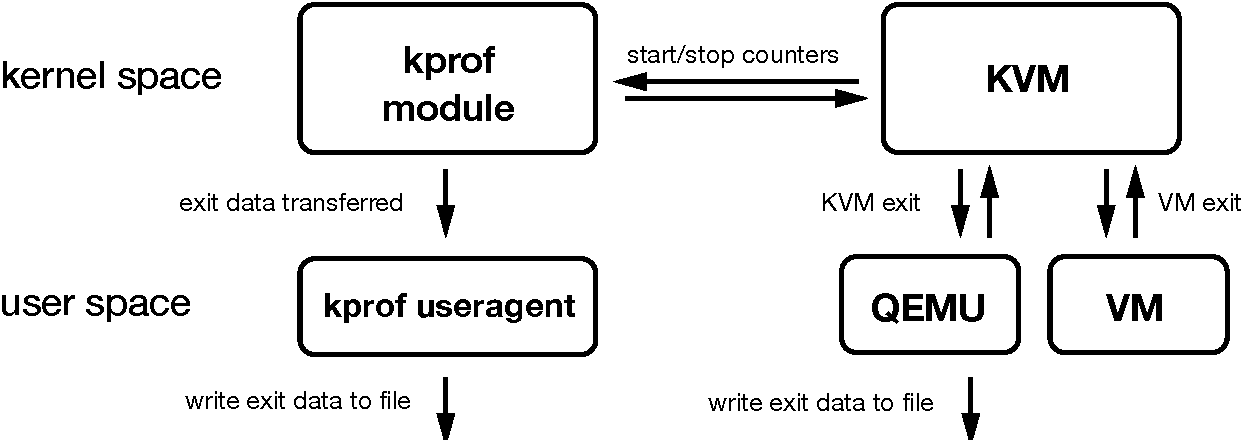
\includegraphics[width=4.5in]{diagram.pdf}
    \caption{System architecture overview composing both userspace and kernel
    space data collection mechanisms.}
    \label{fig:diagram}
\end{figure}


\section{Analysis}

\subsection{iozone and Workload Distribution}
% TODO
\begin{figure}[htp]
    \centering
    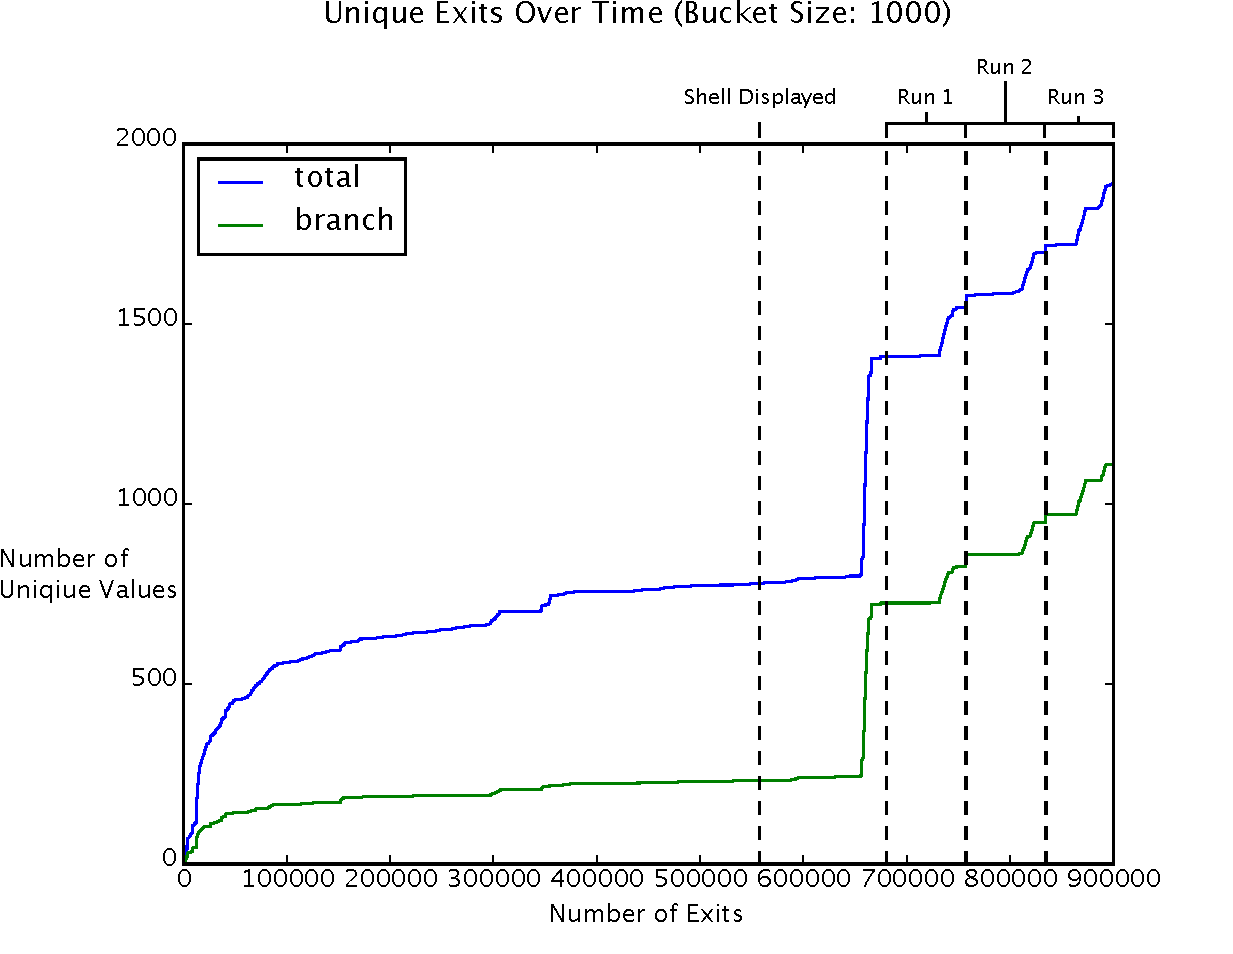
\includegraphics[width=4.5in]{iozone_plot.pdf}
    \caption{Plot of the unique counter values observed over time. The workload
    consists of initial boot of a Linux machine, followed by three succesive
runs of the iozone filesystem benchmark. Here, \textit{bucket size} refers to
a smoothing factor applied to the data. Numbers are placed into buckets of this
size. A bucket size of 1000 means there are buckets of values 0-999, 1000-1999,
etc. Numbers in the same bucket are treated as the same for the creation of this
graph.}
    \label{fig:iozoneplot}
\end{figure}

A visual evaluation of the data as presented in Figure \ref{fig:iozoneplot}
shows that we cannot make an accurate judgement of whether we are seeing a new
wokload purely based on the performance counter data. From this graph, we
observe that the workload manifests as a change in the graph. Additionally, this
graph gives some insights into how the operating system uses the hypervisor. We
observe a high level of entropy at boot and shortly after the shell is displayed
to the user. Runs of the filesystem benchmark increase the number of unique
counters observed, but successive runs do not show an increase by a lesser
delta. From this, we can conclude that while the performance counters are a
valuable metric, they cannot stand alone in detecting certain executions.

This is just one view of the data. Another is to separate the graphs by observed
exit reason. This allows us to interpret the specific nature of the workload.
For the iozone dataset, if we separate the data according to exit reason, there
are many \texttt{HALT} exit reasons occuring during the iozone runs (this exit
reason indicates that the CPU has been paused until the next interrupt occurs).
However, these are sparse during the boot of the operating system. In this case,
the halt instructions might be a sign that there is an IO-heavy operation
occurring or some other device-related operation. These sorts of observations
are interesting for understanding more about the workload.

\subsection{Windows and Linux}
One of the interesting applications of the counter data is to better understand
how Linux and Windows use the hypervisor. We can do this by collecting a sample
of counter values through the kprof module from booting a virtual machine of
both systems.

I collected this data from the aforementioned CentOS VM and a Windows 7 VM, both
running on the same bare metal machine with the same hypervisor and custom QEMU
fork. \footnote{Note: on boot, the Linux VM is able to make a hypercall so as to
    exactly mark when startup is complete, but this is not possible with the
Windows machine.} The data was then fed through a series of scripts to split it
out by exit reason and observe how the number of unique exit reasons grow over
time. This script used a bucket size of 1000 (refer to
Figure~\ref{fig:iozoneplot} for more information on bucket size).

Some interesting trends arise in the data. The two systems have a different
distribution of total exit reasons, with Windows having more EPT\_MISCONFIG and
PENDING\_INTERRUPT exits than Linux. Both boot sequences have high levels of
IO\_INSTRUCTION exits compared other reasons. There are also some differences in
how the exits occur over time.

\begin{figure}[htpb!]
\centering
\subfigure[Windows]{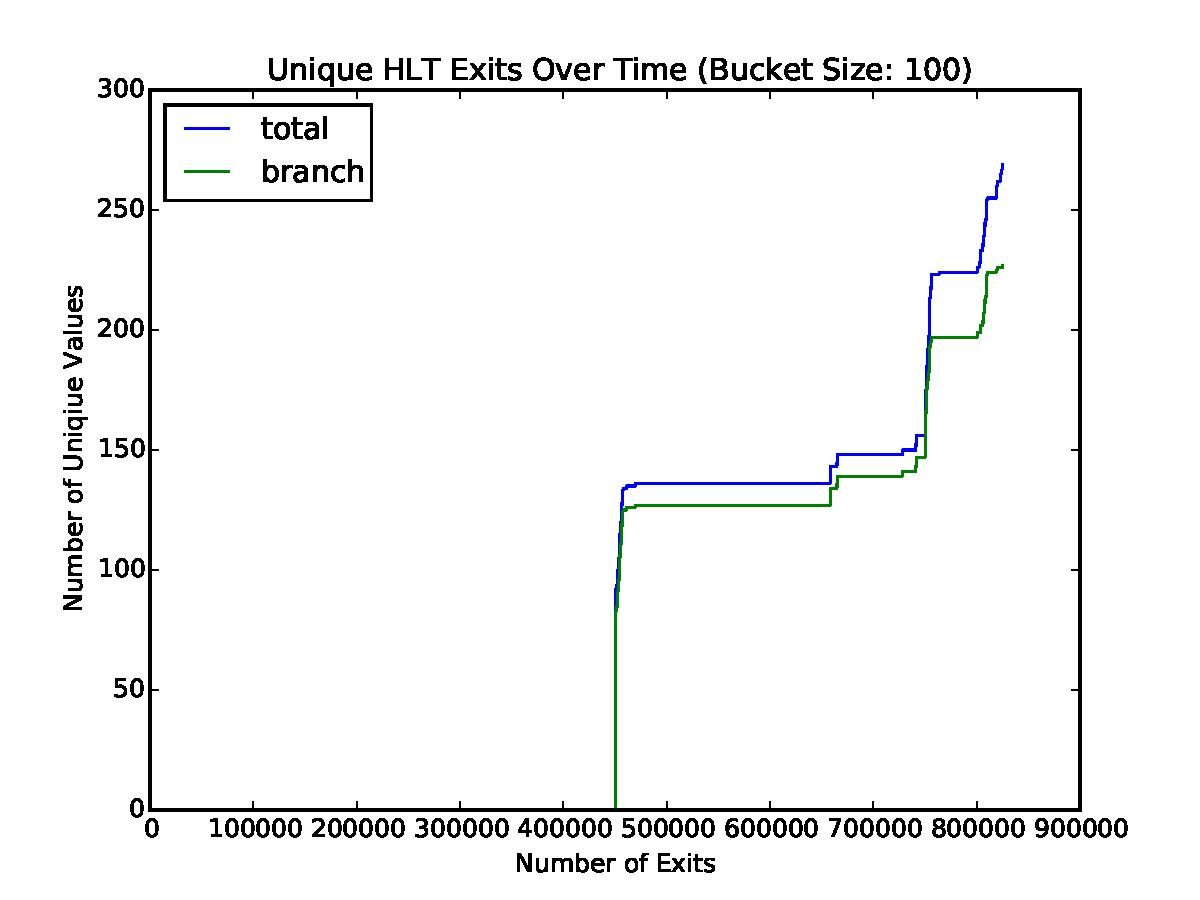
\includegraphics[width=1\textwidth]{hlt_windows.pdf}}\hfill
\subfigure[Linux]{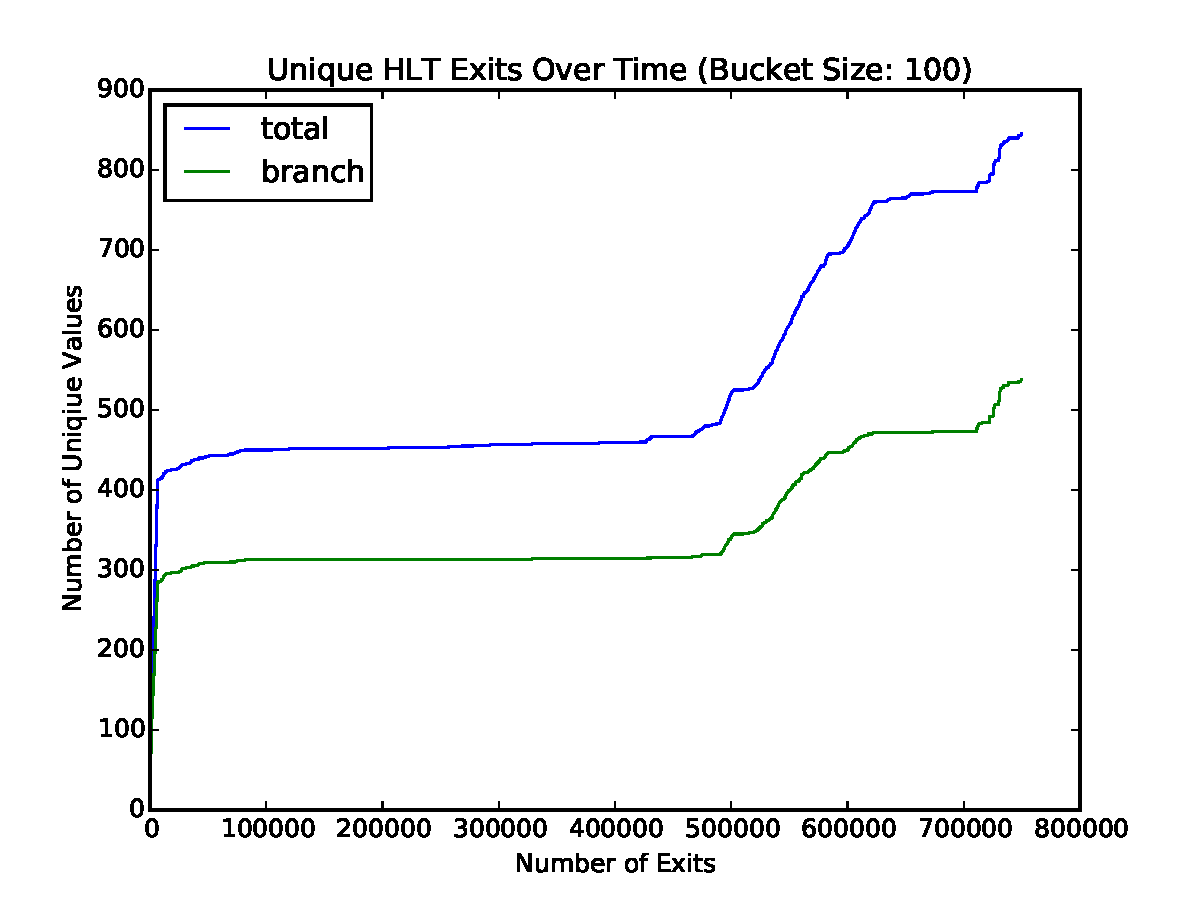
\includegraphics[width=1\textwidth]{hlt_linux.pdf}}\hfill
\caption{Distribution of HLT (halt) exits for Windows and Linux virtual machine
boots. Observe that the number of HLT exits quickly climbs and stabilizes for
Linux, but does so much later in the Windows process. It is difficult to explain
this discrepancy, but it does give some insight that we can use the counter
instrumentation tools to observe differences in how these two operating systems
use the hypervisor when running in a virtual machine.}
\label{fig:winlinhlt}
\end{figure}

\section{Future Work}
Future work will involve building tools around the workload analysis component
of this work. Since the API is already there, this is not too difficult to do
for other developers. They can easily grab the counter data and manipulate it. I
envision many interesting tools stemming from this. One example is a quick tool
to capture the current hypervisor state and graph the next 30 seconds of data to
see if there are any interesting phenomena occurring.

\subsection{Open Questions}
The primary open question is: how can we leverage this existing performance
counter infrastructure and data to create security tools? This is largely the
focus of the hshield % TODO: REF HSHIELD %
paper, which aims to build a new counter containing multiple input sources of
data (such as information about the basic blocks being executed, performance
counter data, and more). From there, a hardware unit can be built to
continuously monitor integrity. Since the overhead of the performance counters
is relatively minimal (due to native support in the CPU), this could be a viable
application of this work.


\section{Conclusion}
Personally, I have learned many interesting things about how virutal machines
operate and how other subsystems of Linux work.

HPCs are an interesting avenue to explore for security purposes, but ultimately
they are more immediately useful as a method of observing how a workload is
distributed and how different systems leverage the hypervisor.


\newpage

% list all references without citing them in the document
\nocite{*}

\bibliography{report}{}
\bibliographystyle{plain}

\end{document}

